\chapter{First Solution (Chapter Title is to be Adapted)}

% This is the third result chapter which presents the first solution of the thesis. 
% The solution is integrated into the overall concept introduced in Chapter 4 and 
% it is technically based on the foundation described in Chapter 5.

% A thesis should provide at least two such solutions. 

\section{Monitoring MVP}

% Sketch
% Which parts are required for a complete solution?
% -> Source, (Collector, Transformer), Sink, Analytics/Visualization
% What requirements have to be fulfilled by a complete solution?
% Which options exist for each part and how do they work together?
% Why were these parts chosen?
% Explanation of solution pipeline
% Extensibility and Scalability

A complete monitoring system requires three main parts: Data sources, data sinks, and the ability
to analyze/visualize the collected data. 
The collected data can be split into three different types: Metrics, Logs, and Traces.
This work only provides a monitoring solution for metrics but logs and traces are still considered
in the development so that they can be added later.

Data sources are the origin of the collected metrics and can be split into two different types
based on how they acquire metrics. The first type is data sources that perform manual instrumentation.
This means that the application source code is amended by code that collects metrics and emits them.
Manual instrumentation is useful for application-specific metrics, like for example, how often a user
uses a certain feature in the application.
The second type is data sources that perform automatic instrumentation.
These data sources collect metrics from applications or the environment without changing any source code.
In contrast to manual instrumentation, automatic instrumentation is limited to collecting
common metrics that are provided by an application and its environment like CPU or memory usage.

Data sinks store the metrics that were collected by the data sources.
It is important to note that some data sinks specialize in which type of data they store
to increase efficiency.

The last part is the analysis and visualization of the collected metrics.

Optionally, a monitoring system might employ additional components like data transformers or collectors.
Data transformers can be used to transform data into different formats, enrich it with additional information
or aggregate it.
Data collectors can be used to buffer metrics that were sent by data sources before they are stored in a data sink,
which decreases the load on the data sink.

\begin{table}[]
\begin{tabular}{l|l}
	& Requirement       			\\
\hline
R1 	& Scalability 					\\
R2 	& Extensibility       			\\
R3 	& Data Types 					\\
R4 	& Open-source       			\\
R5 	& Free commercial use  			\\
R6 	& Cloud agnostic       			\\
R7 	& Integration of Azure data
\end{tabular}
\caption{Requirements for a Monitoring Solution}
\label{tab:requirements}
\end{table}

The components that will be chosen for the monitoring solution must fulfill a few requirements.
These requirements are listed in \ref{tab:requirements}.
Firstly the solution should be scaleable to an arbitrary amount of monitored services and instances.
Secondly, it should be possible to add new and different services in the future.
This means that adding a new service should only require configuration changes and adding new visualizations for the service.
Thirdly, although only metrics are implemented in this solution, it should be possible to extend
the monitoring in the future to also include logs and traces.
Additionally, tools are preferred that are open-source, not bound to a vendor's specific cloud,
and that offer a license for free commercial use.
Overall the solution aims to be as slim as possible. Meaning that it should consist of as few services as possible.
While it is for example possible to use components that specialize in each of the three different data types,
components that support multiple or all three data types are preferred.
Lastly, it has to be possible to integrate data from Azure into the monitoring solution.
This requirement is the result of the underlying use case and the developed demonstrator,
which utilizes Azure.

\begin{table}[]
\begin{tabular}{l|l}
Name 					& Purpose 			\\
\hline
Grafana 				& Visualization		\\
Kibana 					& Visualization		\\
OpenSearch Dashboard 	& Visualization		\\
Prometheus 				& Data sink			\\
ElasticSearch 			& Data sink			\\
OpenSearch 				& Data sink			\\
OpenTelemetry 			& Data source		\\
Jaeger 					& All-in-one		\\
Apache SkyWalking 		& All-in-one
\end{tabular}
\caption{Potential Tools for the monitoring solution}
\label{tab:potential_tools}
\end{table}

The tools that were considered for the monitoring solution are listed in \ref{tab:potential_tools}.

Jaeger can immediately be ruled out as it only supports traces.
With the same reasoning, Prometheus can also be ruled out as it only supports metrics.
ElasticSearch was up until recently commercially free to use which is no longer the case.
OpenSearch is being developed as an open-source, free-to-use alternative with the goal
of offering the same feature set. Kibana is a visualization tool specifically developed for
ElasticSearch, which means that it is also being ruled out as ElasticSearch won't be used.
While Apache SkyWalking offers an all-in-one solution from data source to visualization,
it does not seem like it can integrate the monitoring data from Azure.
This leaves only Grafana, OpenSearch, and OpenTelemetry.
Between the OpenSearch Dashboard and Grafana, Grafana is chosen as it offers a wide range
of plugins to connect to different data sources in the future. One of these plugins also
directly allows the integration of data from Azure.
In conclusion, Grafana will be used for visualization and analysis, OpenSearch as the data sink without its Dashboard,
and OpenTelemetry as the data source.

Because OpenTelemetry exports metrics in its OpenTelemetry Protocol format,
which is not yet supported for direct ingestion by OpenSearch,
an additional tool, called Data Prepper has to be employed.
Data Prepper is a data transformer and part of the OpenSearch project that can convert
data from OpenTelemetry into a format that can be ingested into OpenSearch.
In the future, when OpenSearch supports the OpenTelemetry Protocol, this component can be removed.

As per the recommendations of the OpenSearch project, the OpenSearch Collector will also be used
in the monitoring solution. The OpenSearch Collector acts as a buffer between the data sources
and the data sink. It can also be used for certain automatic instrumentation tasks.

The resulting SystemPlusSoftware architecture can be seen in \ref{fig:sps_monitoring_mvp}.

\begin{figure}[h]
	\centering
	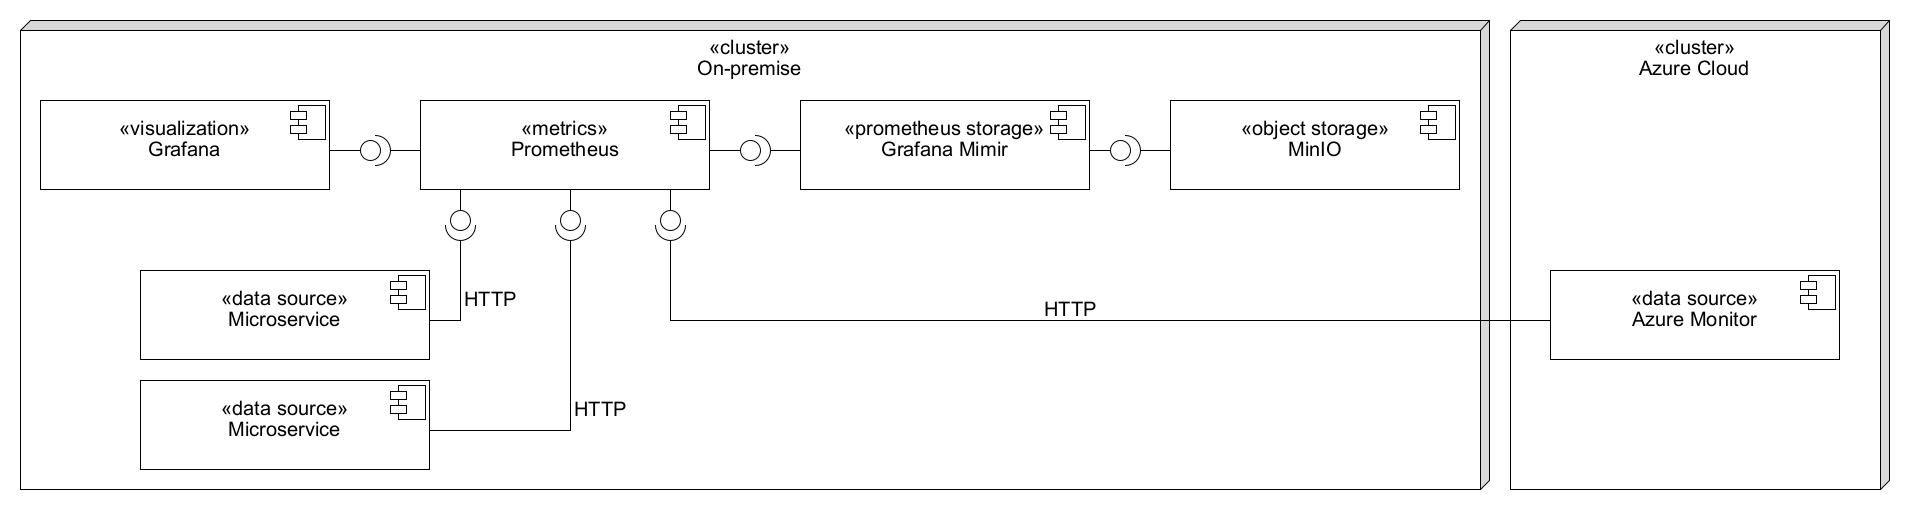
\includegraphics[width=\textwidth]{figures/sps_monitoring_mvp.png}
	\caption{SystemPlusSoftware Monitoring MVP}
	\label{fig:sps_monitoring_mvp}
\end{figure}

\begin{figure}[h]
	\centering
	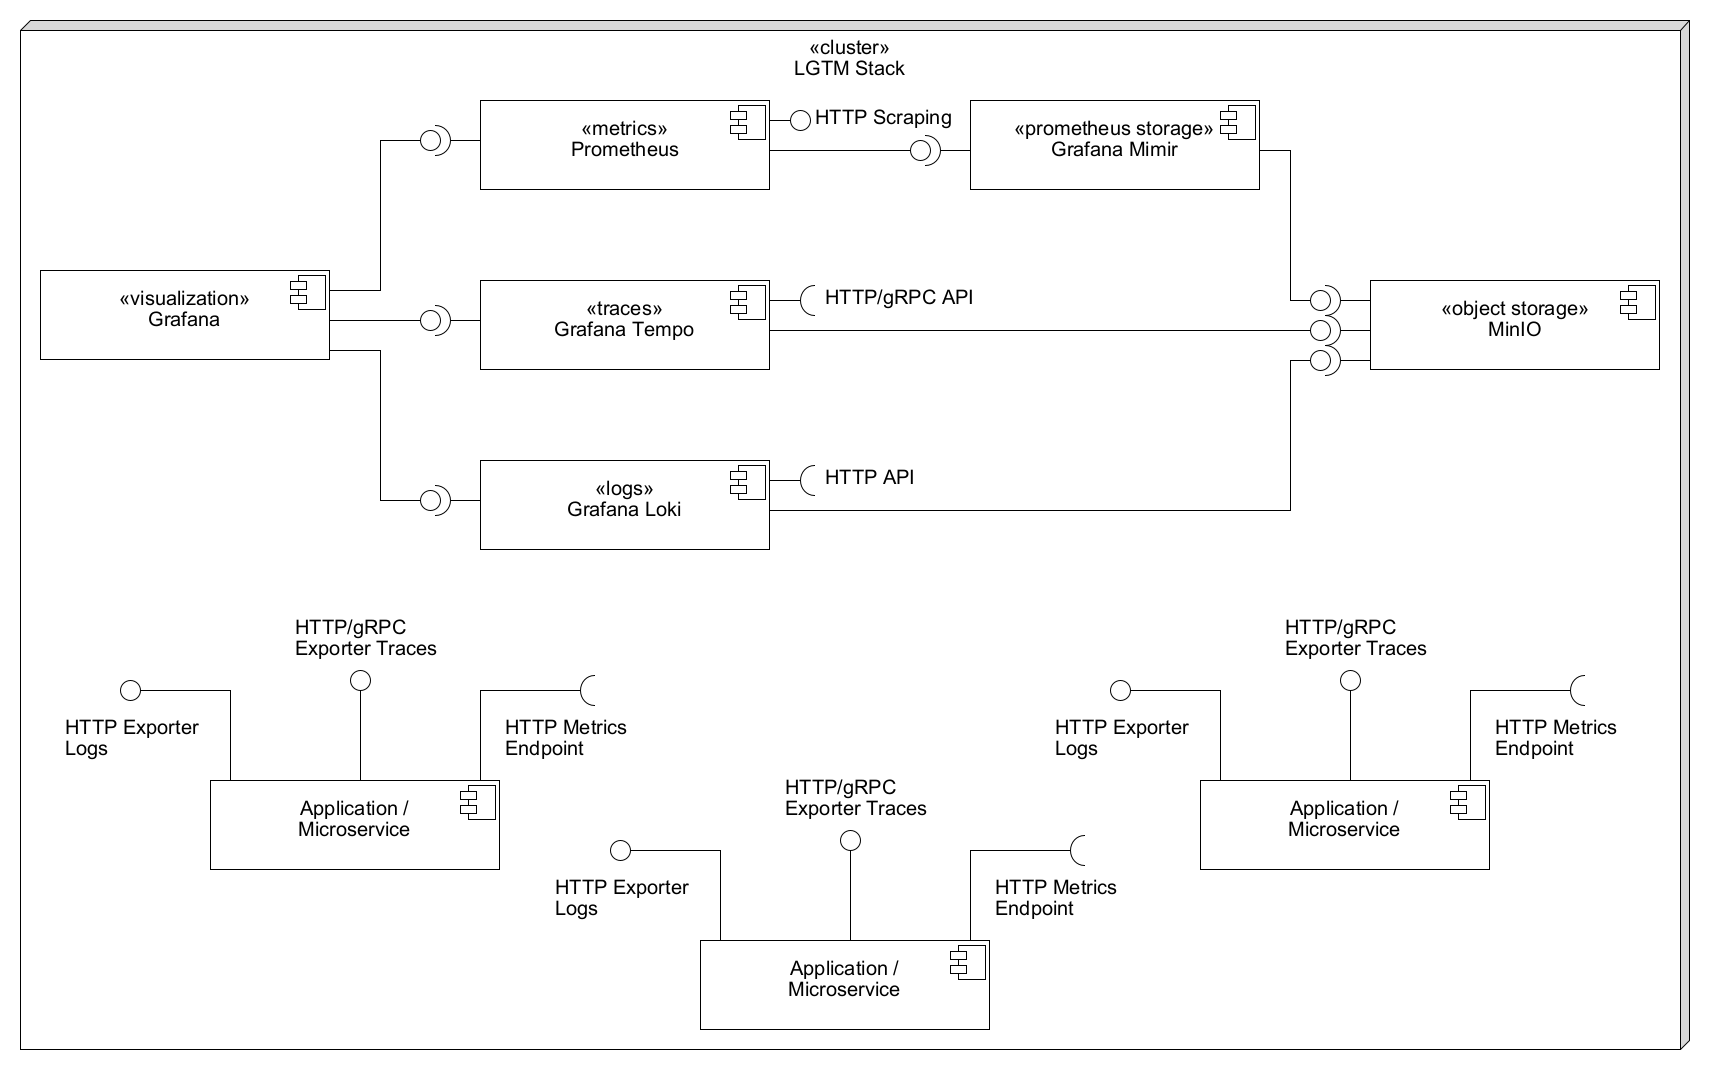
\includegraphics[width=\textwidth]{figures/lgtm_stack.png}
	\caption{LGTM Stack}
	\label{fig:lgtm_stack}
\end{figure}